\documentclass{article}
%\documentclass[a4paper,10pt,draft]{thesis}
\usepackage{physics,amsmath, amsfonts, siunitx, amssymb, graphicx, slashed,subcaption}
\usepackage[utf8]{inputenc}
\usepackage[margin=1in]{geometry}
\usepackage[hidelinks]{hyperref}
\usepackage{xr-hyper}
\newcommand{\n}[1]{\nu_{#1}}
\newcommand{\na}{\nu_\alpha}
\newcommand{\nb}{\nu_\beta}
\newcommand{\ana}{\bar{\nu}_\alpha}
\newcommand{\an}[1]{\bar{\nu}_{\text{#1}}}
\newcommand{\anb}{\bar{\nu}_\beta}
\renewcommand{\a}{\alpha}
\renewcommand{\b}{\beta}
\newcommand{\ab}{\alpha\beta}


\renewcommand{\ne}{\nu_e}
\newcommand{\nm}{\nu_\mu}
\newcommand{\nt}{\nu_\tau}
\newcommand{\ns}{\nu_s}

\newcommand{\ane}{\bar{\nu}_e}
\newcommand{\anm}{\bar{\nu}_\mu}
\newcommand{\ant}{\bar{\nu}_\tau}
\newcommand{\ans}{\bar{\nu}_s}

\newcommand{\nee}{\nu_e \to \nu_e}
\newcommand{\nem}{\nu_e \to \nu_\mu}
\newcommand{\net}{\nu_e \to \nu_\tau}
\newcommand{\nes}{\nu_e \to \nu_s}

\newcommand{\nme}{\nu_\mu \to \nu_e}
\newcommand{\nmm}{\nu_\mu \to \nu_\mu}
\newcommand{\nmt}{\nu_\mu \to \nu_\tau}
\newcommand{\nms}{\nu_\mu \to \nu_s}



\newcommand{\Pee}{P_{e  e}}
\newcommand{\Pem}{P_{e  \mu}}
\newcommand{\Pet}{P_{e  \tau}}
\newcommand{\Pes}{P_{e  s}}

\newcommand{\Pme}{P_{\mu  e}}
\newcommand{\Pmm}{P_{\mu\mu}}
\newcommand{\Pmt}{P_{\mu  \tau}}
\newcommand{\Pms}{P_{\mu  s}}


\newcommand{\Pte}{P_{P_{\tau e}}}
\newcommand{\Ptm}{P_{\tau  \mu}}
\newcommand{\Ptt}{P_{\tau  \tau}}
\newcommand{\Pts}{P_{\mu  s}}

\newcommand{\Paeae}{P_{\bar{e}  \bar{e}}}
\newcommand{\Paeam}{P_{\bar{e}  \bar{\mu}}}
\newcommand{\Paeat}{P_{\bar{e}  \bar{\tau}}}
\newcommand{\Paeas}{P_{\bar{e}  \bar{s}}}

\newcommand{\Pamae}{P_{\bar{\mu}  \bar{e}}}
\newcommand{\Pamam}{P_{\bar{\mu}  \bar{\mu}}}
\newcommand{\Pamat}{P_{\bar{\mu}  \bar{\tau}}}
\newcommand{\Pamas}{P_{\bar{\mu}  \bar{s}}}


\newcommand{\Patae}{P_{\bar{\tau}  \bar{e}}}
\newcommand{\Patam}{P_{\bar{\tau}  \bar{\mu}}}
\newcommand{\Patat}{P_{\bar{\tau}  \bar{\tau}}}
\newcommand{\Patas}{P_{\bar{\mu}  \bar{s}}}

\renewcommand{\th}[1][]{%
  \theta\ifx\\#1\\\else_\text{#1}\fi
}
\newcommand{\thm}[1][]{%
  \theta^\text{M}\ifx\\#1\\\else_\text{#1}\fi
}
\renewcommand{\t}[1]{\text{{#1}}}
\newcommand{\avg}[1]{\left\langle {#1} \right \rangle}
\newcommand*{\dm}[1][]{%
  \Delta m^2\ifx\\#1\\\else_\text{#1}\fi
}
\newcommand{\zreco}{\cos{(\theta_z^{reco})}}
\newcommand{\ztrue}{\cos{(\theta_z^{true})}}
\newcommand{\z}{\cos{(\theta_z)}}
\newcommand{\Ereco}{E^{reco}}
\newcommand{\Etrue}{E^{true}}
\newcommand{\Aeff}{A^\text{eff}}
\newcommand{\emm}{\epsilon_{\mu\mu}}
\newcommand{\emt}{\epsilon_{\mu\tau}}
\newcommand{\eet}{\epsilon_{e\tau}}
\newcommand{\eem}{\epsilon_{e\mu}}
\newcommand{\ett}{\epsilon_{\tau\tau}}
\newcommand{\ep}{\epsilon^\prime}

\newcommand{\zreco}{\ensuremath{\cos{(\theta_z^{reco})}}}
\newcommand{\ztrue}{\ensuremath{\cos{(\theta_z^{true})}}}
\newcommand{\emm}{\ensuremath{\varepsilon_{\mu\mu}}}
\newcommand{\emt}{\ensuremath{\varepsilon_{\mu\tau}}}
\newcommand{\ett}{\ensuremath{\varepsilon_{\tau\tau}}}
\newcommand{\ep}{\ensuremath{\varepsilon^\prime}}
\usepackage{physics,amsmath, amsfonts, siunitx, amssymb,cite, graphicx}
\usepackage[utf8]{inputenc}
\usepackage{hyperref}
\begin{document}
\section{Methodology}

In this part, we use the publically available DeepCore data sample~\cite{DC2019data} which is an updated version of what was used by the 
IceCube collaboration in an $\nu_\mu$ disapprearance analysis~\cite{DC2018mudisappearance}.

The detector systematics include ice absorption and scattering, and overall, lateral, and head-on optical efficiencies of the DOMs. 
They are applied as correction factors using the best-fit points from the DeepCore 2019 $\nu_\tau$ appearance 
analysis~\cite{DC2019tauappearance}.

The data events include 14901 track-live events and 26001 cascade-like events, both divided into eight 
$ \log_{10}E^{reco} \in [0.75,1.75]$ bins, and eight $\zreco \in [-1,1]$ bins.

The neutrino flux at the detector is calculated by propagating atmospheric neutrino flux~\cite{hondapaper} through the Earth by solving the 
Schrödinger equation for varying density. The Earth density profile is taken from the PREM~\cite{PREM}. The oscillation parameters are from the
best-fit in the global analysis in~\cite{nufit}: $\theta_{12} = \SI{33.44}{\degree},\, \theta_{13} = \SI{8.57}{\degree},\, \Delta m^2_{21} =  \SI{7.42}{\electronvolt^2}$, and we 
marginalize over $\Delta m^2_{31}$ and $\theta_{23}$.
The oscillation probability $P_{\alpha \beta}$ then acts as a weight, yielding the propagated flux at detector level for flavor $\beta$ as 
\begin{align}\label{eq:propFlux}
    \Phi_\beta = \sum_\alpha \frac{\dd^2 \phi_\alpha}{\dd E^t \dd \cos{\theta^t_z}} P_{\alpha\beta}\,,
\end{align}
where we sum over the initial lepton flavors $\alpha \in {e,\mu, \bar{e}, \bar{\mu}}$.
The event rate for each bin reads
\begin{align}\label{eq:events}
    N_{ij} &= T \int_{(\cos{\theta_z^r})_i}^{(\cos{\theta_z^r})_{i+1}} \dd \cos{\theta^r_z} \int_{E^r_{j}}^{E^r_{j+1}} \dd E^r \int_0^\pi R(\theta^r,\theta^t) \dd \cos{\theta^t} \int_0^\infty R(E^r,E^t) \dd E^t \nonumber\\
        &\times \left[ \sum_\beta \Phi_\beta  A^\text{eff}_\beta\right]\,,
\end{align}
where $T$ is the live time of the detector, and $A^\text{eff}_\beta$ its effective area for flavor $\beta$. $R(x^r,x^t)$ is a Gaussian resolution function, 
which is responsible for the smearing between the reconstructed and true parameters $x^r$ and $x^t$, respectively. It takes the form 
\begin{align}
    R(x^r, x^t) = \frac{1}{\sqrt{2\pi} \sigma_{x^r}} \exp\left[\frac{(x^r-\mu(x^t))^2}{2\sigma_{x^r}^2}\right]\,.
\end{align}
Assuming no bias in the reconstruction, the mean of the Gaussian can be taken as $\mu(x^t) = x^t$. As seen in Fig.~\ref{fig:IC_MC_counts}, the distribution of 
simulated events is skewed. Instead, we assume a log-normal distribution between $E^{true}$ and $E^{reco}$, and train a Gaussian Process Regressor on the dataset, from which
we can extract a predicted mean and standard deviation for each $E^{reco}$. We then sample values from this distribution to yield 
the points of $E^{true}$ at which to integrate over. 

In Icecube, the zenith angle resolution for track-like events is less than $\SI{2}{\degree}$, making $\ztrue$ coincide with $\zreco$ for our study~\cite{IC2020}.
\begin{figure}[!tb]
    \begin{center}
       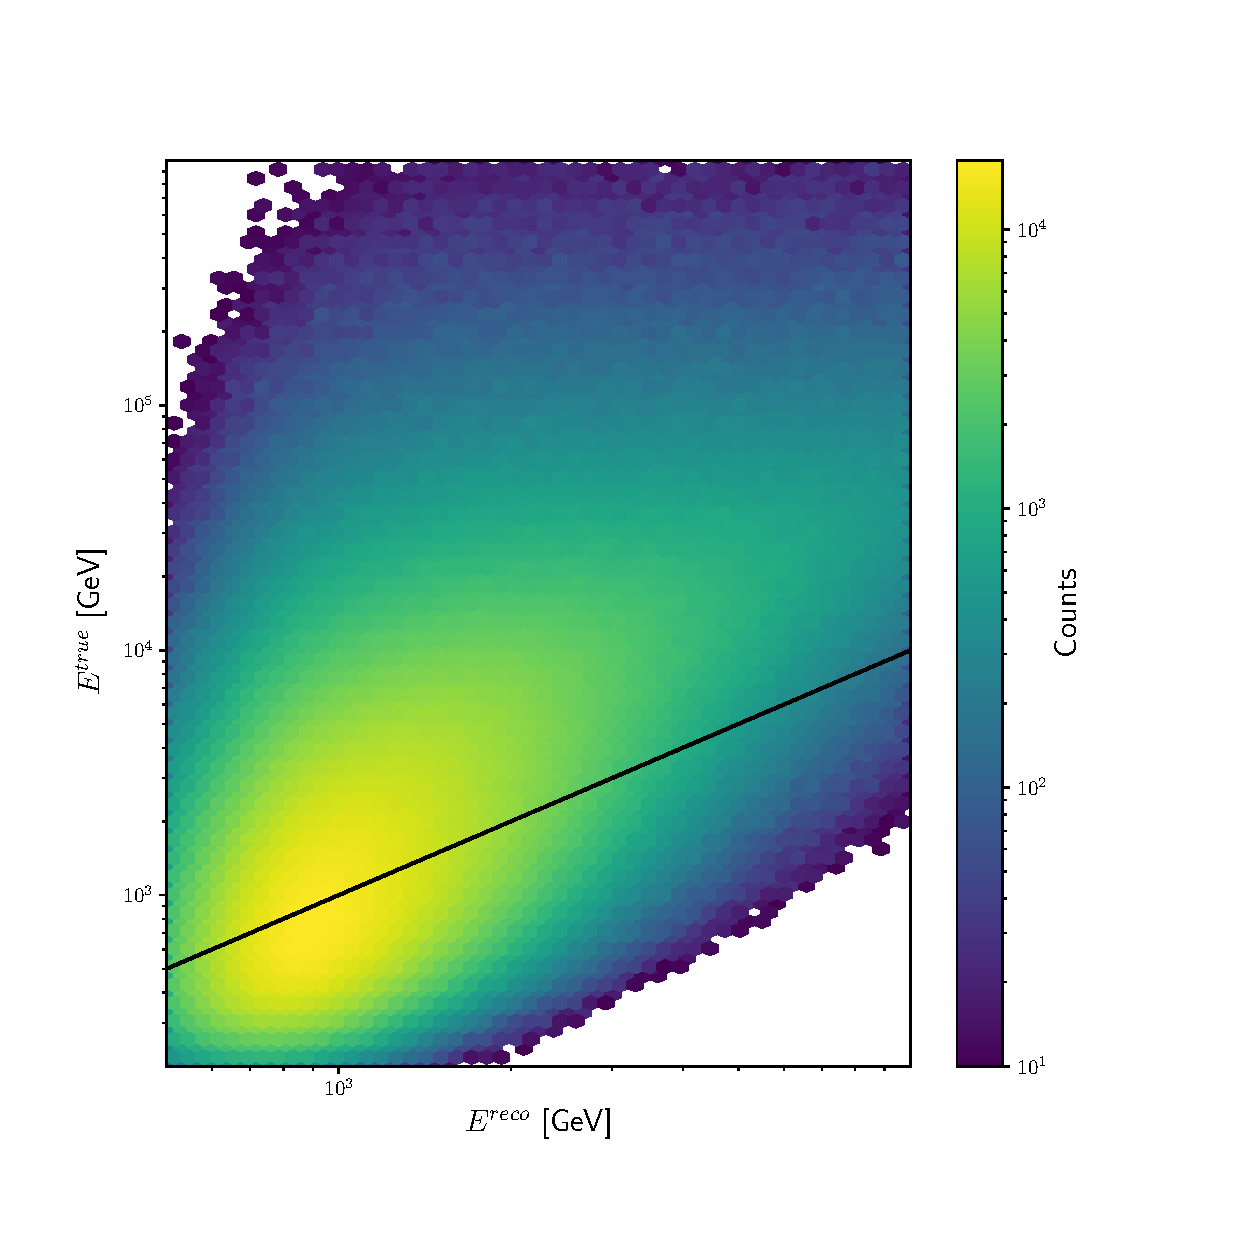
\includegraphics[width=0.48\linewidth]{figures/IC_MC_counts.eps}
    \end{center}
    \caption{Relationship between the true and reconstructed muon energy in the IceCube MC sample}\label{fig:IC_MC_counts}
 \end{figure}

Given a Monte Carlo simulation with weights $w_{k\beta}$, we can construct the event count as
\begin{align}\label{eq:MCevents}
    N_{ijk} &= C_{ijk}\sum_{\beta}w_{ijk,\beta} \Phi_\beta\,,
\end{align}
where $C_{k\beta}$ is the correction factor from the detector systematic uncertainty and $\Phi_\beta$ is defined as Eq.~\ref{eq:propFlux}. We have now substituted the effect of the Gaussian smearing 
by treating the reconstructed and true quantities as a migration matrix. 

We define our $\chi^2$ as
\begin{align} \label{eq:chisq}
    \chi^{2}(\hat{\theta},\alpha,\beta)=\sum_{ijk} \frac{\left(N^\text{th}+N^{\mu_{atm}}-N^\text{data}\right)_{ijk}^{2}}
    {\left(\sigma^\text{data}\right)_{ijk}^{2}+\left(\sigma_{\nu + \mu_\text{atm}}^\text{uncor}\right)_{ijk}^{2}}+ 
    \frac{(1-\alpha)^2}{\sigma_\alpha^2} + \frac{\beta^2}{\sigma_\beta^2}\,
\end{align}
where we minimize over the model parameters $\hat{\theta} \in \{\Delta m_{31}^2, \theta_{23}, \ep, \emt\}$, and the penalty terms $\alpha$ and $\beta$.
$N_{ijk}^\text{th}$ is the expected number of events from theory, and $N_{ijk}^\text{data}$ is the observed number of events in that bin. 
The event count takes the form
\begin{align}
    N^\text{th}_{ijk} = \alpha\left[1+\beta \zreco_i \right] N_{ijk}(\hat{\theta})\,,
\end{align}
with $N_{ijk}(\hat{\theta})$ from Eq.~\ref{eq:MCevents}. $N_{ijk}^{\mu_{atm}}$ is the muon background, which is left to float freely in the analysis.
We use $\sigma_\alpha = 0.25$ as the atmospheric flux normalization error, and $\sigma_\beta = 0.04$ as the zenith angle slope error~\cite{hondapaper}. 
The observed event number has an associated Poissonian uncertainty $\sigma_{i}^\text{data} = \sqrt{N_{i}^\text{data}}$. 
The term $\sigma_{\nu + \mu_\text{atm}}^\text{uncor}$ accounts for both uncertanties in the finite MC statistics and in the data-driven 
muon background estimate~\cite{DC2019data}.

\bibliographystyle{elsarticle-num}
\bibliography{article}
\end{document}


